\documentclass[11pt, a4paper]{article}

\usepackage[margin=1in]{geometry}
\usepackage{amsmath, amssymb}
\usepackage{graphicx}
\usepackage{booktabs}
\usepackage{subcaption}
\usepackage{parskip}
\usepackage[hidelinks]{hyperref}

% Works whether compiled from reports/, project root, or Overleaf (plots/ or root)
\graphicspath{{../results/plots/}{results/plots/}{plots/}{./}}

\title{\textbf{Project 6: Irrelevant Variables and the Curse of Dimensionality}}
\author{Course: MAC 312 -- Foundations of Data Science \\[4pt]
        \textit{Name (ID Number)}}
\date{\today}

\begin{document}
\maketitle

\begin{abstract}
In high-dimensional data, many features often have no real link to the target label. In this report, we study how adding such independent noise features affects four classifiers: $k$-Nearest Neighbours (KNN), Gaussian Kernel Density Estimation (KDE), a Regularized Gaussian classifier (QDA), and L2 Logistic Regression. Using controlled synthetic experiments, we vary the ambient dimension $d$, training sample size $n$, feature scales, and informative dimension $r$. We find that distance-based methods (KNN and KDE) break down quickly as $d$ grows because pairwise distances concentrate around the same value. Increasing the sample size $n$ helps parametric models recover near-optimal accuracy, while local methods improve very slowly. We also show that standardizing features helps when noise variables have much larger variance than the signal, fails to remove equal-scale noise, and actually hurts when the signal already has a larger scale. Only supervised feature weighting or feature selection brings performance back to the oracle level.
\end{abstract}

% =====================================================================
\section{Introduction and Problem Setup}

In real datasets, we rarely know beforehand which variables actually help predict the label and which ones are just noise. Adding extra irrelevant features does not change the true relationship between the useful features and the label, so an ideal model should not get worse. In practice, however, extra dimensions spread data points far apart and distort Euclidean distances. This effect is known as the \textit{curse of dimensionality}.

\subsection{Data-Generating Model}
To study this cleanly, we generate synthetic binary classification data $x = (z, u) \in \mathbb{R}^d$ with balanced classes $P(y=0) = P(y=1) = 0.5$:
\begin{itemize}
    \item \textbf{Informative features} $z \in \mathbb{R}^r$:
    \[
        z \mid (y = 0) \sim \mathcal{N}(-\delta \mathbf{1}_r, \sigma_z^2 I_r), \qquad
        z \mid (y = 1) \sim \mathcal{N}(+\delta \mathbf{1}_r, \sigma_z^2 I_r).
    \]
    \item \textbf{Irrelevant noise features} $u \in \mathbb{R}^{d-r}$:
    \[
        u \sim \mathcal{N}(0, \sigma_u^2 I_{d-r}), \qquad u \perp (z, y).
    \]
\end{itemize}
Because $u$ is completely independent of both $z$ and $y$, the true posterior probability depends only on $z$:
\[
    \log \frac{P(y=1 \mid x)}{P(y=0 \mid x)}
    = \log \frac{P(y=1 \mid z)}{P(y=0 \mid z)}
    = \frac{2\delta}{\sigma_z^2} \sum_{j=1}^{r} z_j.
\]

\subsection{Keeping Problems Comparable Across $r$ and Scale}
When we later change the number of informative features $r$ or their scale $\sigma_z$, we do not want the problem itself to become easier or harder. If $\delta$ stayed fixed while $r$ increased, the distance between the two class means, $\|\mu_1 - \mu_0\|_2 = 2\delta\sqrt{r}$, would grow and make larger $r$ unfairly easy. To avoid this, we set
\[
    \delta = \frac{\mu_0}{\sqrt{r}} \sigma_z, \qquad \text{with } \mu_0 = 1.2.
\]
If we define the single summary score $s(z) = \frac{1}{\sigma_z \sqrt{r}} \sum_{j=1}^r z_j$, then $s(z) \mid (y=0) \sim \mathcal{N}(-\mu_0, 1)$ and $s(z) \mid (y=1) \sim \mathcal{N}(+\mu_0, 1)$. Thus, the best possible error rate (the \textbf{Bayes optimal error}) is always
\[
    \text{Bayes Error} = \Phi(-\mu_0) = \Phi(-1.2) \approx 0.1151 \text{ (11.51\%)},
\]
no matter what values we pick for $r$, $d$, $\sigma_z$, or $\sigma_u$. The Bayes optimal log-loss also stays the same across every experiment.

\subsection{Classifiers, Tuning, and Evaluation Metrics}
Every experiment uses independent training, validation ($n_{\text{val}} = 500$), and test ($n_{\text{test}} = 1000$) sets, repeated over 5 random seeds (42 to 46). All hyperparameters are chosen strictly on the validation set:
\begin{enumerate}
    \item \textbf{KNN:} Euclidean $k$-nearest neighbours with $k \in \{1, 3, 5, 7, 11, 15, 21, 31, 51\}$, tuned by validation error (with log-loss as tie-breaker). Class probability is the fraction of neighbours in class 1.
    \item \textbf{Gaussian KDE:} Estimates each class density $p(x \mid y=c)$ with an isotropic Gaussian kernel of bandwidth $h \in \{0.2, 0.5, 1, 2, 3, 5, 10, 20, 50, 100\}$ (computed in log-space for numerical stability), tuned by validation log-loss.
    \item \textbf{Regularized Gaussian (QDA):} Fits class means and shrinks each class sample covariance toward a scaled identity matrix: $\Sigma_c^{\text{reg}} = (1-\alpha) S_c + \alpha \frac{\operatorname{Tr}(S_c)}{d} I_d$, with $\alpha \in \{0, 0.01, 0.05, 0.1, 0.2, 0.5, 0.8, 1.0\}$ tuned by validation log-loss.
    \item \textbf{L2 Logistic Regression:} Linear model with L2 regularization strength $C \in \{10^{-4}, 10^{-3}, \dots, 10^2\}$, tuned by validation log-loss.
\end{enumerate}

On the test set, we record four quantities:
\begin{itemize}
    \item \textbf{Classification error rate:} fraction of misclassified test points.
    \item \textbf{Predictive log-loss:} $-\frac{1}{n_{\text{test}}} \sum_i \big[y_i \log \hat{p}_i + (1-y_i)\log(1-\hat{p}_i)\big]$, with predicted probabilities clipped to $[10^{-15}, 1-10^{-15}]$.
    \item \textbf{Nearest and farthest distances ($D_{\text{near}}$, $D_{\text{far}}$):} for each test point, its Euclidean distance to the closest and farthest training point, averaged over the test set.
    \item \textbf{Distance contrast ($C$):} defined per test point and averaged over the test set as
    \[
        C = \frac{D_{\text{far}} - D_{\text{near}}}{D_{\text{near}}}.
    \]
    A large contrast means close points are much nearer than far points; a contrast close to 0 means all points lie at almost the same distance.
\end{itemize}

% =====================================================================
\section{Why High Dimensions Hurt Distances (Geometric Intuition)}

Before looking at the experimental plots, it helps to look at the math behind squared Euclidean distances. For two independent points $x = (z, u)$ and $x' = (z', u')$, their squared distance splits into a signal part and a noise part:
\[
    \|x - x'\|^2 = \|z - z'\|^2 + \|u - u'\|^2.
\]

\subsection{Moments of the Noise Term and Distance Concentration}
Each noise difference satisfies $u_j - u'_j \sim \mathcal{N}(0, 2\sigma_u^2)$ independently for $j = 1, \dots, d-r$. Therefore, $\frac{\|u - u'\|^2}{2\sigma_u^2} \sim \chi^2(d-r)$. Using the standard mean and variance of a chi-squared distribution, we get:
\[
    \mathbb{E}\big[\|u - u'\|^2\big] = 2(d - r)\sigma_u^2, \qquad
    \operatorname{Var}\big(\|u - u'\|^2\big) = 8(d - r)\sigma_u^4.
\]
Notice that the mean grows linearly with $(d - r)$, while the standard deviation $\sqrt{8(d-r)}\,\sigma_u^2$ only grows as $\sqrt{d-r}$. So the relative spread around the mean shrinks as
\[
    \frac{\operatorname{SD}(\|u - u'\|^2)}{\mathbb{E}[\|u - u'\|^2]} = \sqrt{\frac{2}{d - r}} \longrightarrow 0 \quad \text{as } d \to \infty.
\]
Because the relative spread goes to zero, almost all points end up sitting on a thin shell at roughly the same distance ($\approx \sqrt{2d}\sigma_u$), and the distance contrast $C$ collapses toward 0.

\subsection{Same-Class vs.\ Opposite-Class Distance Gap}
Now include the informative coordinates $z$ (with $\delta = \frac{\mu_0}{\sqrt{r}}\sigma_z$):
\begin{align*}
    \mathbb{E}\big[\|x - x'\|^2 \mid y = y'\big] &= 2r\sigma_z^2 + 2(d - r)\sigma_u^2, \\
    \mathbb{E}\big[\|x - x'\|^2 \mid y \neq y'\big] &= 4\mu_0^2 \sigma_z^2 + 2r\sigma_z^2 + 2(d - r)\sigma_u^2.
\end{align*}
The average squared-distance gap between opposite-class and same-class points is fixed at $4\mu_0^2 \sigma_z^2$ (it does not grow with $d$ or $r$). Meanwhile, the random noise standard deviation is $\sqrt{8(d - r)}\,\sigma_u^2$. Taking their ratio gives a simple distance signal-to-noise ratio:
\[
    \text{SNR}_{\text{dist}}
    = \frac{4\mu_0^2 \sigma_z^2}{\sqrt{8(d - r)}\,\sigma_u^2}
    = \frac{\sqrt{2}\,\mu_0^2}{\sqrt{d - r}} \left(\frac{\sigma_z}{\sigma_u}\right)^2.
\]
When $d - r$ is large or when $\sigma_u \gg \sigma_z$, $\text{SNR}_{\text{dist}}$ becomes much smaller than 1. Random fluctuations in the noise coordinates easily drown out the true class gap. As a result, a test point's ``nearest'' neighbours are almost just as likely to belong to the wrong class as the right class, causing KNN and KDE to fail.

% =====================================================================
\section{Experiment 1: Increasing Ambient Dimension ($d$)}

In Experiment 1, we hold the informative features fixed at $r = 2$, $n_{\text{train}} = 500$, and $\sigma_z = \sigma_u = 1.0$, and increase the total dimension $d \in \{2, 5, 10, 20, 50, 100, 200\}$ by adding pure noise variables.

\begin{table}[htbp]
\centering
\small
\caption{Experiment 1 results (mean $\pm$ std over 5 seeds) for selected ambient dimensions $d$ ($r=2, n_{\text{train}}=500$).}
\label{tab:exp1}
\begin{tabular}{rlcccc}
\toprule
$d$ & Classifier & Error Rate & Log-Loss & $D_{\text{near}}$ & Contrast $C$ \\
\midrule
2   & Gaussian   & $0.1132 \pm 0.0051$ & $0.2710 \pm 0.0085$ & 0.130  & 84.15 \\
    & GaussianKDE & $0.1140 \pm 0.0048$ & $0.2798 \pm 0.0114$ & 0.130  & 84.15 \\
    & KNN        & $0.1174 \pm 0.0044$ & $0.4623 \pm 0.2610$ & 0.130  & 84.15 \\
    & LogReg     & $0.1132 \pm 0.0061$ & $0.2712 \pm 0.0085$ & 0.130  & 84.15 \\
\midrule
20  & Gaussian   & $0.1156 \pm 0.0029$ & $0.2770 \pm 0.0071$ & 3.856  & 1.464 \\
    & GaussianKDE & $0.1838 \pm 0.0041$ & $0.3991 \pm 0.0099$ & 3.856  & 1.464 \\
    & KNN        & $0.1352 \pm 0.0100$ & $0.3934 \pm 0.0120$ & 3.856  & 1.464 \\
    & LogReg     & $0.1198 \pm 0.0029$ & $0.2895 \pm 0.0049$ & 3.856  & 1.464 \\
\midrule
50  & Gaussian   & $0.1222 \pm 0.0082$ & $0.2863 \pm 0.0112$ & 7.477  & 0.725 \\
    & GaussianKDE & $0.1602 \pm 0.0046$ & $0.4767 \pm 0.0025$ & 7.477  & 0.725 \\
    & KNN        & $0.1472 \pm 0.0122$ & $0.4727 \pm 0.0027$ & 7.477  & 0.725 \\
    & LogReg     & $0.1306 \pm 0.0083$ & $0.3020 \pm 0.0150$ & 7.477  & 0.725 \\
\midrule
200 & Gaussian   & $0.1400 \pm 0.0042$ & $0.3358 \pm 0.0134$ & 17.430 & 0.305 \\
    & GaussianKDE & $0.2298 \pm 0.0211$ & $0.5736 \pm 0.0084$ & 17.430 & 0.305 \\
    & KNN        & $0.2168 \pm 0.0313$ & $0.5687 \pm 0.0097$ & 17.430 & 0.305 \\
    & LogReg     & $0.1534 \pm 0.0093$ & $0.3956 \pm 0.0094$ & 17.430 & 0.305 \\
\bottomrule
\end{tabular}
\end{table}

\begin{figure}[htbp]
    \centering
    \begin{subfigure}[b]{0.48\textwidth}
        \centering
        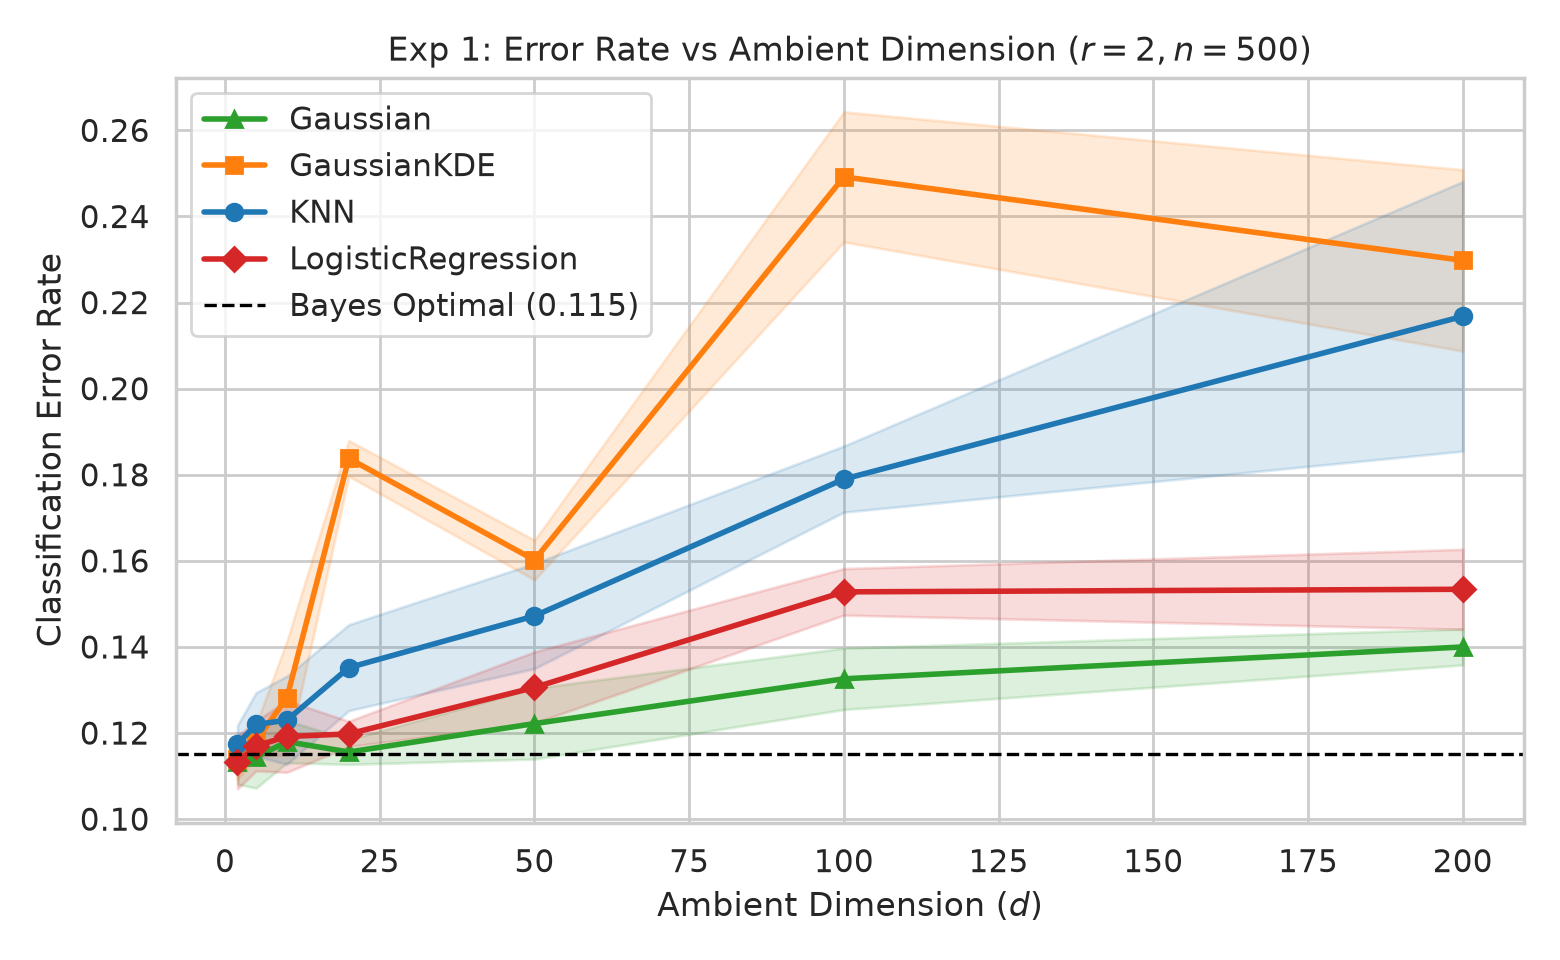
\includegraphics[width=\textwidth]{exp1_error_vs_ambient_dim.png}
        \caption{Classification error rate vs.\ $d$.}
    \end{subfigure}
    \hfill
    \begin{subfigure}[b]{0.48\textwidth}
        \centering
        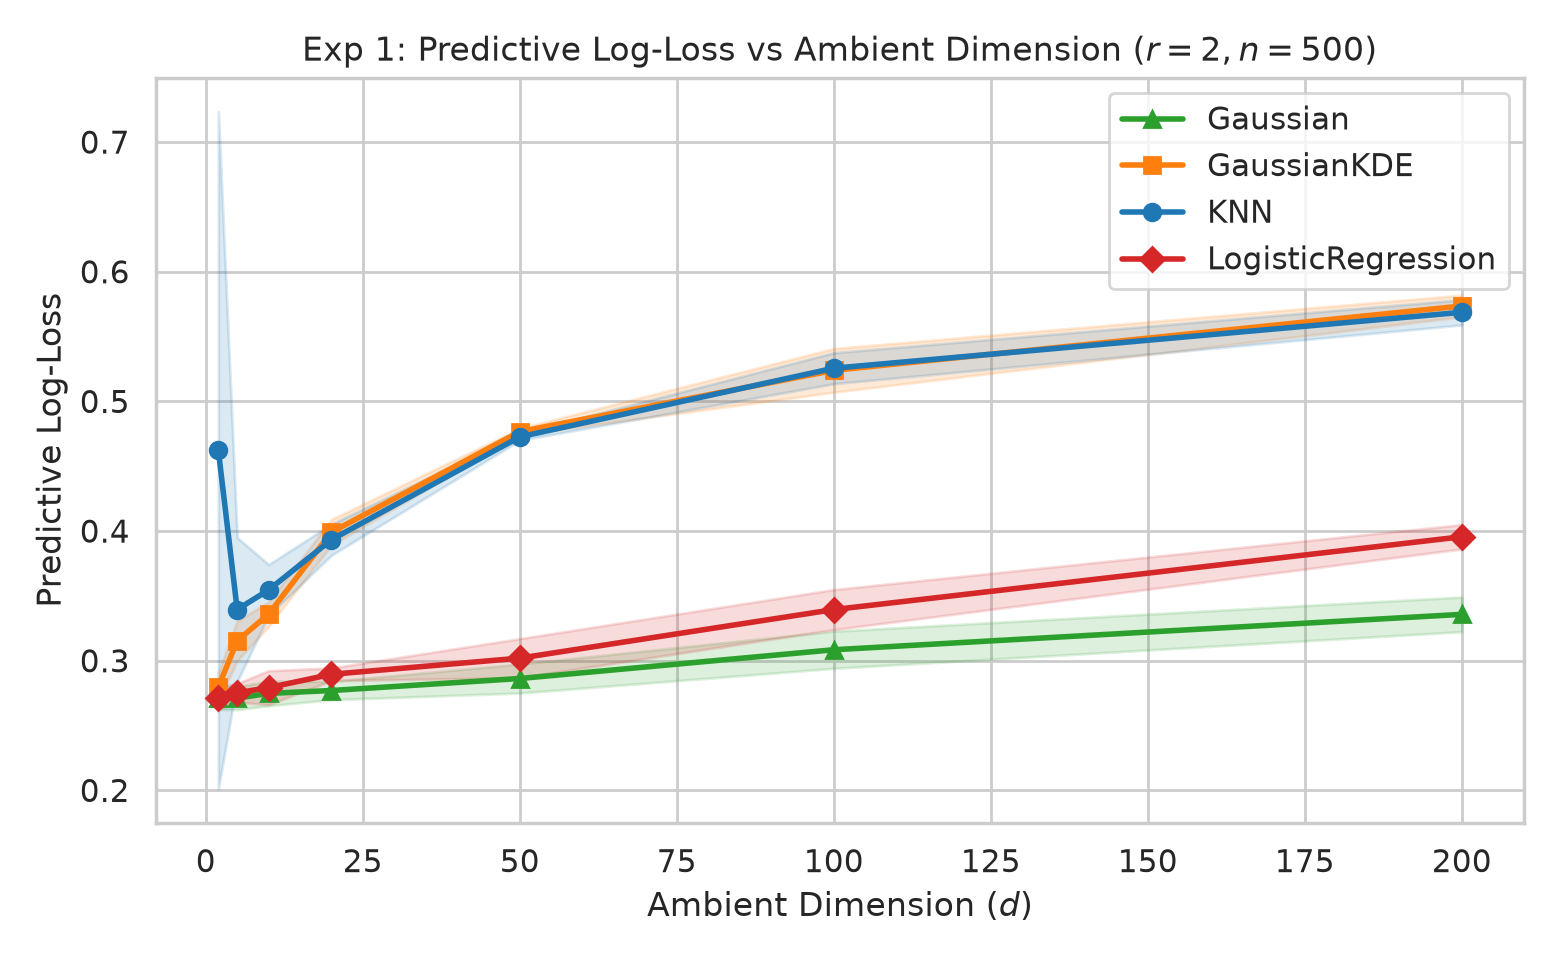
\includegraphics[width=\textwidth]{exp1_log_loss_vs_ambient_dim.png}
        \caption{Predictive log-loss vs.\ $d$.}
    \end{subfigure}
    \caption{Experiment 1: Effect of adding irrelevant variables ($r=2, n_{\text{train}}=500$).}
    \label{fig:exp1_perf}
\end{figure}

\begin{figure}[htbp]
    \centering
    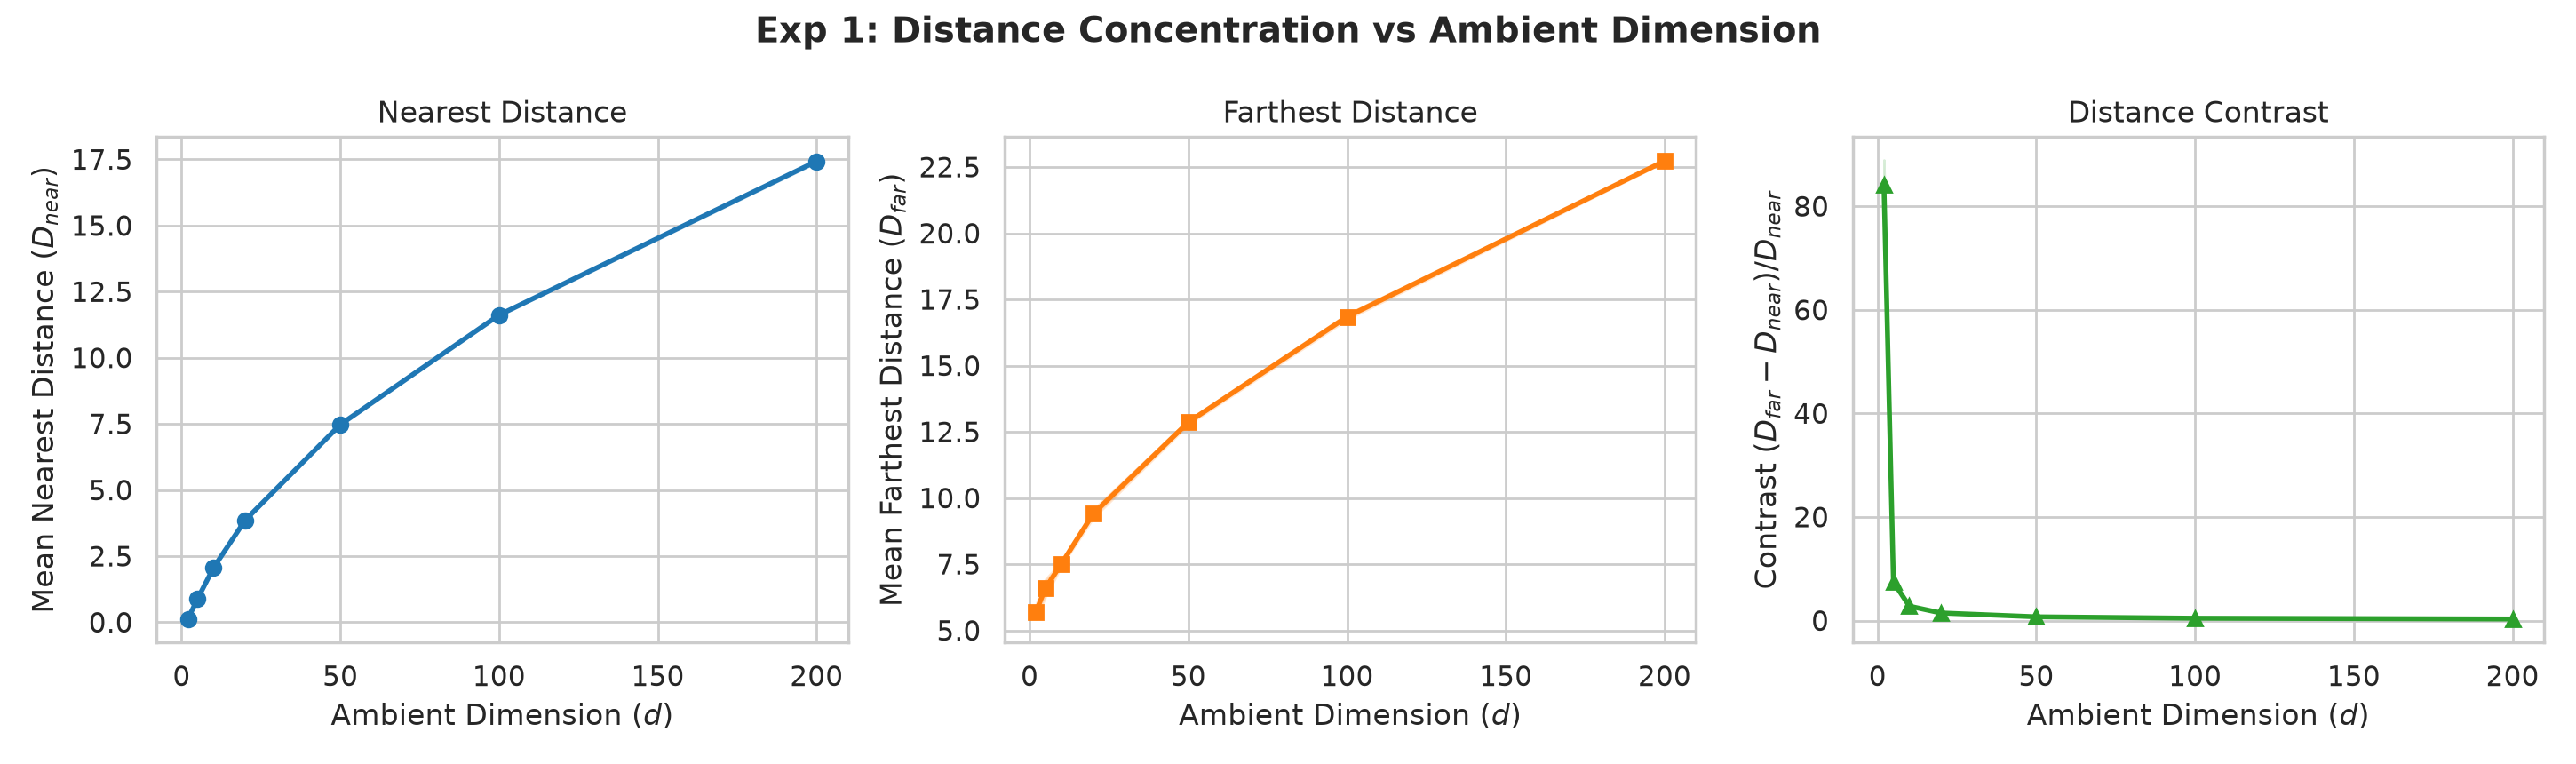
\includegraphics[width=\textwidth]{exp1_distance_concentration.png}
    \caption{Experiment 1: Nearest distance $D_{\text{near}}$, farthest distance $D_{\text{far}}$, and distance contrast $C$ as $d$ grows.}
    \label{fig:exp1_dist}
\end{figure}

\textbf{Observations:}
\begin{itemize}
    \item \textbf{Distance concentration is dramatic:} As shown in Figure~\ref{fig:exp1_dist} and Table~\ref{tab:exp1}, $D_{\text{near}}$ grows from $0.13$ at $d=2$ to $17.43$ at $d=200$, while distance contrast $C$ drops from $84.15$ down to $0.305$. At $d=200$, the farthest point in the dataset is only about 30\% farther away than the very closest neighbour.
    \item \textbf{Local methods degrade fastest:} As seen in Figure~\ref{fig:exp1_perf}, at $d=2$ all four models match the Bayes optimal error of $11.5\%$. By $d=200$, KNN rises to $21.7\%$ error (log-loss $0.569$) and Gaussian KDE rises to $23.0\%$ error (log-loss $0.574$). (Note: KNN has high log-loss variance at $d=2$ because raw vote fractions $m/k$ occasionally predict $0$ or $1$ when $k$ is small, which gets penalized heavily by log-loss.)
    \item \textbf{Parametric models hold up much better:} Regularized Gaussian ($14.0\%$ error, $0.336$ log-loss) and L2 Logistic Regression ($15.3\%$ error, $0.396$ log-loss) stay much closer to Bayes optimal. Logistic regression shrinks the weights of noise coordinates toward zero, and covariance shrinkage keeps the Gaussian model from overfitting noisy sample covariances.
\end{itemize}

% =====================================================================
\section{Experiment 2: Increasing Training Sample Size ($n$)}

Next, we fix $r = 2$, $d = 50$ (48 noise variables), and $\sigma_z = \sigma_u = 1.0$, and vary the training size $n_{\text{train}} \in \{100, 250, 500, 1000, 2500, 5000\}$ to check whether simply collecting more data fixes the problem.

\begin{table}[htbp]
\centering
\small
\caption{Experiment 2 results (mean $\pm$ std over 5 seeds) across training sizes $n_{\text{train}}$ ($d=50, r=2$).}
\label{tab:exp2}
\begin{tabular}{rlcccc}
\toprule
$n_{\text{train}}$ & Classifier & Error Rate & Log-Loss & $D_{\text{near}}$ & Contrast $C$ \\
\midrule
100  & Gaussian    & $0.1504 \pm 0.0054$ & $0.3522 \pm 0.0065$ & 7.895 & 0.568 \\
     & GaussianKDE & $0.2388 \pm 0.0388$ & $0.5176 \pm 0.0377$ & 7.895 & 0.568 \\
     & KNN         & $0.1884 \pm 0.0226$ & $0.5710 \pm 0.0167$ & 7.895 & 0.568 \\
     & LogReg      & $0.1626 \pm 0.0136$ & $0.3777 \pm 0.0229$ & 7.895 & 0.568 \\
\midrule
1000 & Gaussian    & $0.1206 \pm 0.0026$ & $0.2789 \pm 0.0090$ & 7.311 & 0.783 \\
     & GaussianKDE & $0.1340 \pm 0.0102$ & $0.4755 \pm 0.0071$ & 7.311 & 0.783 \\
     & KNN         & $0.1408 \pm 0.0114$ & $0.4459 \pm 0.0080$ & 7.311 & 0.783 \\
     & LogReg      & $0.1194 \pm 0.0062$ & $0.2889 \pm 0.0111$ & 7.311 & 0.783 \\
\midrule
5000 & Gaussian    & $0.1146 \pm 0.0073$ & $0.2717 \pm 0.0076$ & 6.946 & 0.938 \\
     & GaussianKDE & $0.1228 \pm 0.0027$ & $0.4717 \pm 0.0050$ & 6.946 & 0.938 \\
     & KNN         & $0.1402 \pm 0.0055$ & $0.4051 \pm 0.0069$ & 6.946 & 0.938 \\
     & LogReg      & $0.1174 \pm 0.0072$ & $0.2754 \pm 0.0075$ & 6.946 & 0.938 \\
\bottomrule
\end{tabular}
\end{table}

\begin{figure}[htbp]
    \centering
    \begin{subfigure}[b]{0.48\textwidth}
        \centering
        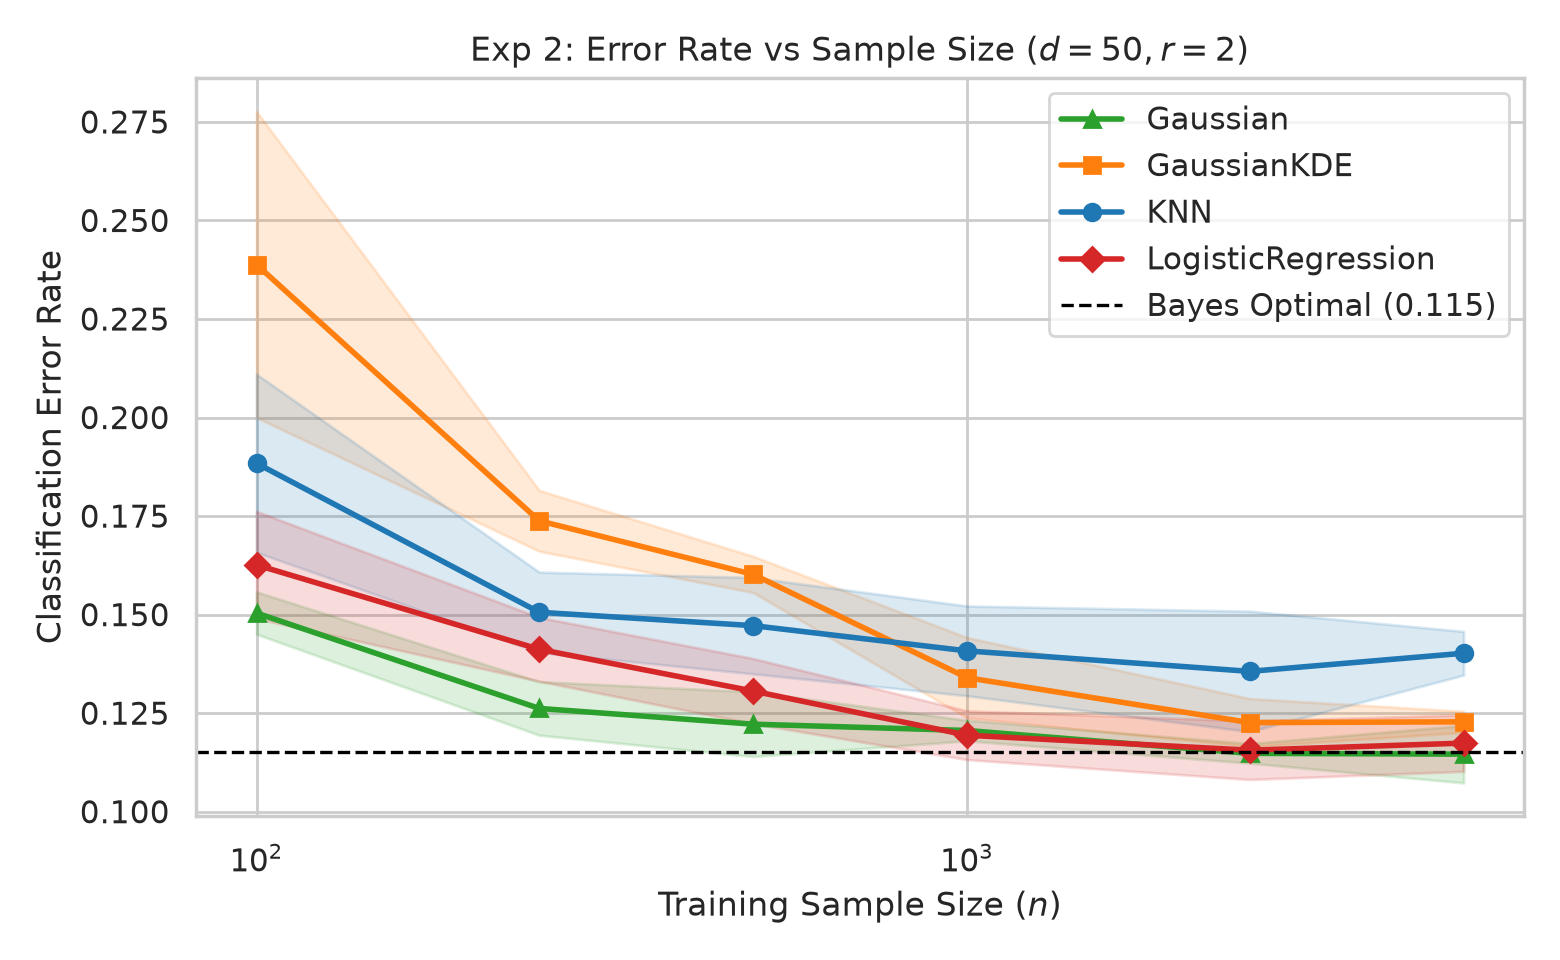
\includegraphics[width=\textwidth]{exp2_error_vs_sample_size.png}
        \caption{Classification error rate vs.\ $n$.}
    \end{subfigure}
    \hfill
    \begin{subfigure}[b]{0.48\textwidth}
        \centering
        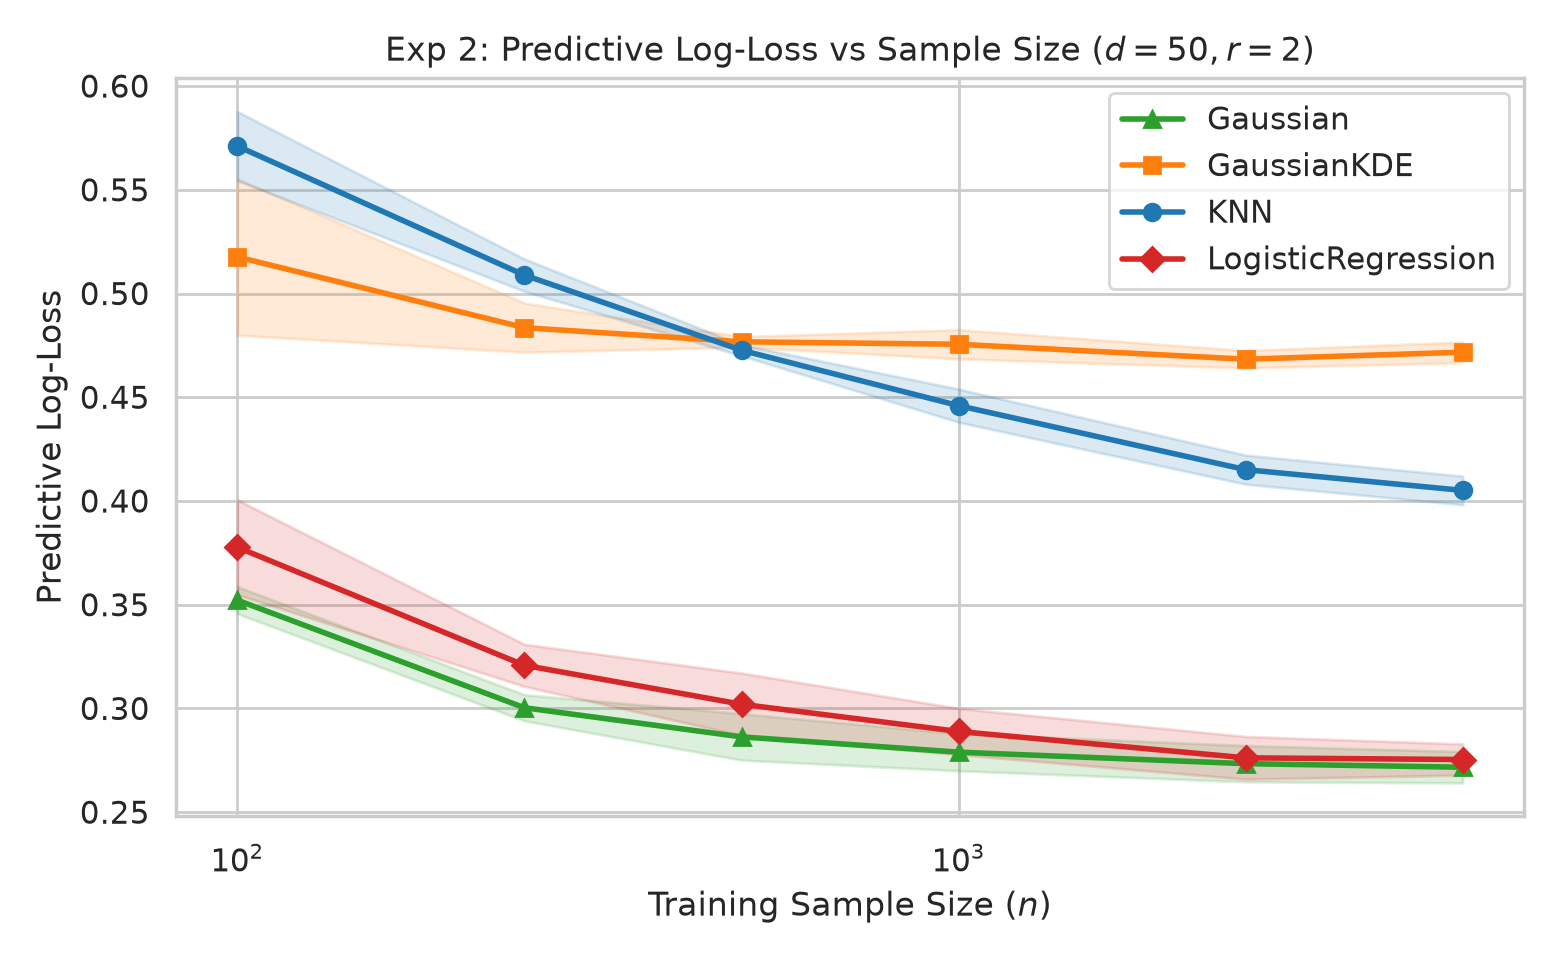
\includegraphics[width=\textwidth]{exp2_log_loss_vs_sample_size.png}
        \caption{Predictive log-loss vs.\ $n$.}
    \end{subfigure}
    \caption{Experiment 2: Effect of increasing training sample size $n$ at $d=50, r=2$.}
    \label{fig:exp2_perf}
\end{figure}

\begin{figure}[htbp]
    \centering
    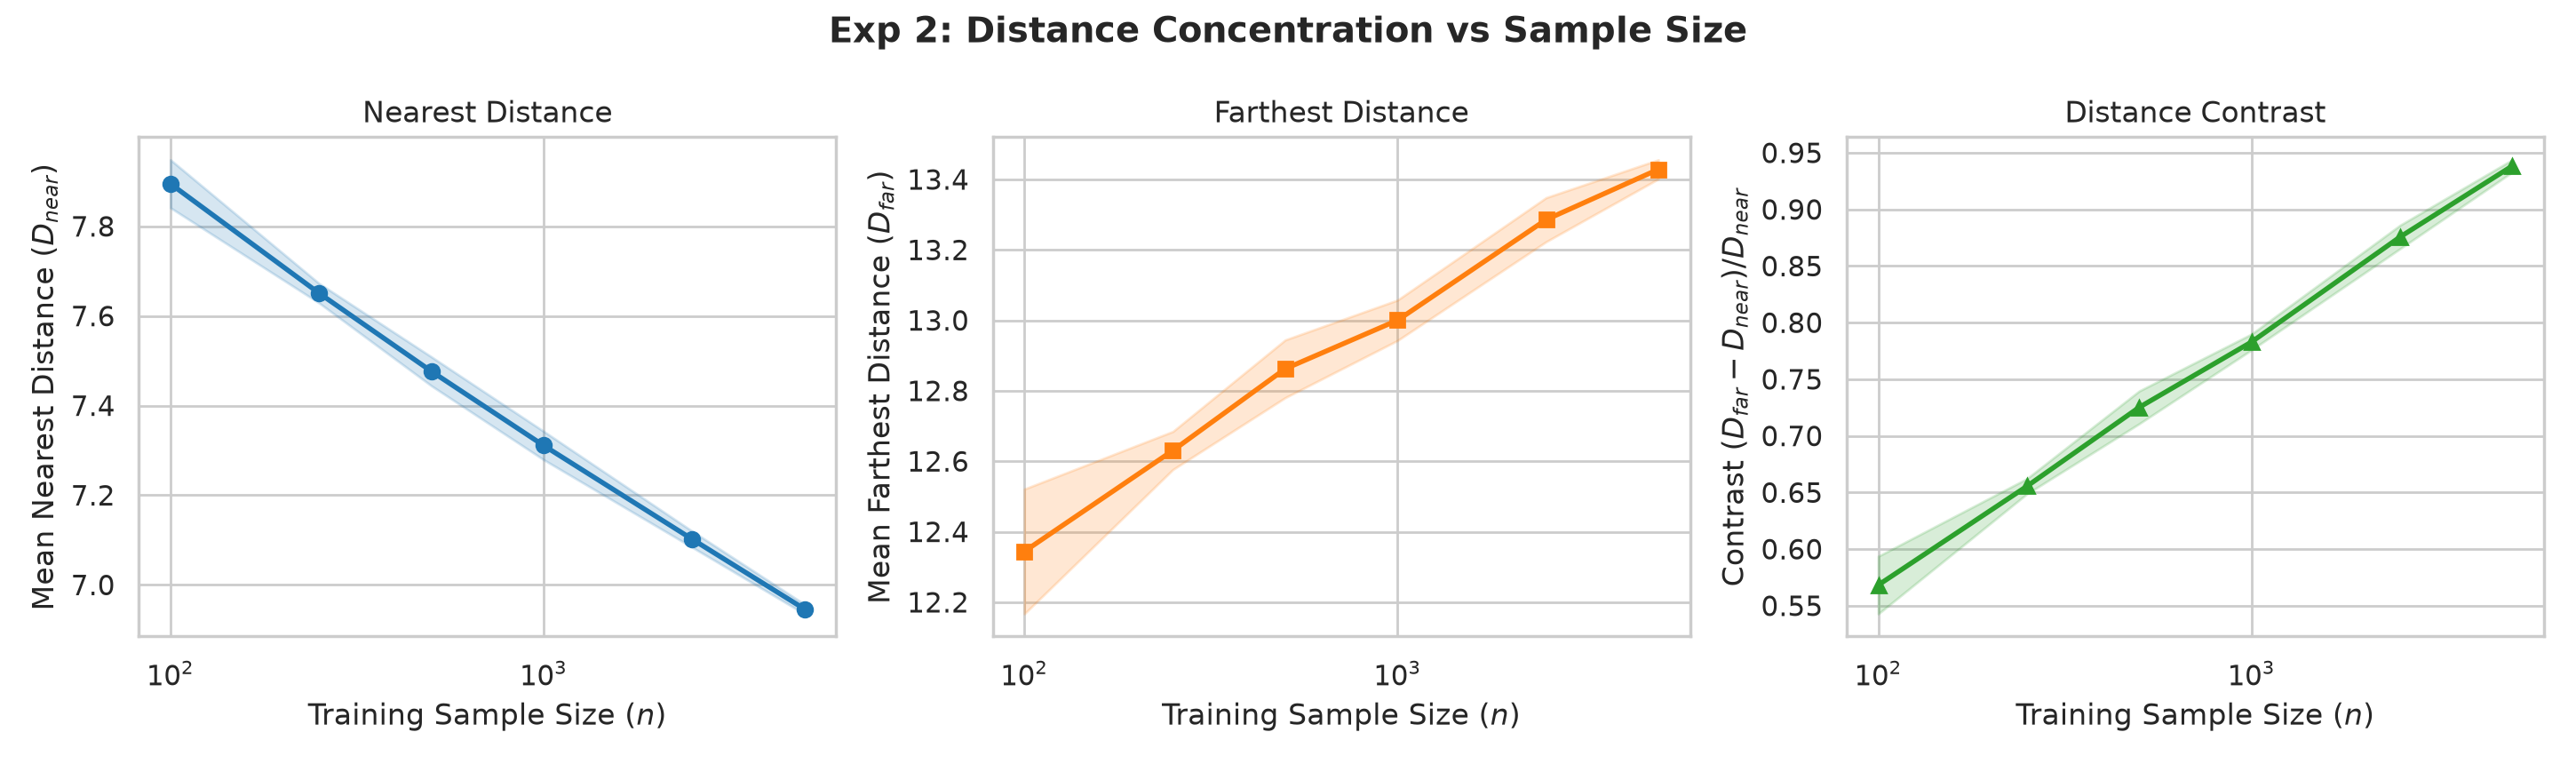
\includegraphics[width=\textwidth]{exp2_distance_vs_sample_size.png}
    \caption{Experiment 2: Distance geometry ($D_{\text{near}}$, $D_{\text{far}}$, and contrast $C$) as $n$ increases by $50\times$.}
    \label{fig:exp2_dist}
\end{figure}

\textbf{Observations:}
\begin{itemize}
    \item \textbf{Parametric models reach Bayes optimal:} As shown in Table~\ref{tab:exp2} and Figure~\ref{fig:exp2_perf}, increasing $n$ by $50\times$ (from 100 to 5000) lets Regularized Gaussian ($15.0\% \to 11.5\%$) and Logistic Regression ($16.3\% \to 11.7\%$) converge right to the Bayes floor of $11.5\%$, with log-loss dropping to $\approx 0.27$.
    \item \textbf{Local methods improve very slowly:} Even with $50\times$ more data, $D_{\text{near}}$ barely moves (from $7.90$ down to $6.95$) and contrast $C$ stays below $1.0$ (Figure~\ref{fig:exp2_dist}). At $n=5000$, KNN is still stuck at $14.0\%$ error ($0.405$ log-loss), and KDE log-loss barely budges ($0.472$). In 50 dimensions, filling space densely enough for local neighbourhoods to work would need an astronomically large number of samples (exponential in $d$).
\end{itemize}

% =====================================================================
\section{Experiment 3: Unequal Feature Scales and Standardization Regimes}

In Experiment 3, we fix $r = 2$, $d = 50$, and $n_{\text{train}} = 500$, and test three different feature-scale regimes (all keeping the exact same Bayes error of $11.51\%$):
\begin{enumerate}
    \item \textbf{Noise-Dominated:} $\sigma_z = 1, \sigma_u = 10$ (noise features have $100\times$ larger variance).
    \item \textbf{Equal-Scale:} $\sigma_z = 1, \sigma_u = 1$.
    \item \textbf{Signal-Dominated:} $\sigma_z = 10, \sigma_u = 1$ (informative features have $100\times$ larger variance).
\end{enumerate}

In each regime, we compare five preprocessing pipelines (all fitted on training data only):
\begin{itemize}
    \item \textbf{Raw:} features used as-is.
    \item \textbf{Standardized:} each feature shifted to mean 0 and scaled to unit variance.
    \item \textbf{Weighted:} standardize, then multiply each coordinate by $\sqrt{w_j}$ where $w_j$ is proportional to its training ANOVA $F$-score (normalized to average weight 1).
    \item \textbf{Selected:} standardize, then keep only the top-$k$ features by training ANOVA $F$-score (\texttt{SelectKBest}), where $k \in \{1, 2, 3, 5, 10, 20, 50\}$ is tuned on the validation set.
    \item \textbf{Oracle:} diagnostic baseline given only the true informative features $z$.
\end{itemize}

\begin{table}[htbp]
\centering
\small
\caption{Experiment 3 mean test error rates and distance contrast $C$ across the three scale regimes ($d=50, r=2, n_{\text{train}}=500$).}
\label{tab:exp3}
\begin{tabular}{llccccc}
\toprule
Regime & Pipeline & KNN & KDE & Gaussian & LogReg & Contrast $C$ \\
\midrule
Noise-Dominated & Raw          & 0.4906 & 0.4852 & 0.4764 & 0.1384 & 0.73 \\
($\sigma_z=1, \sigma_u=10$) & Standardized & 0.1852 & 0.2048 & 0.1390 & 0.1324 & 0.71 \\
                & Weighted     & 0.1210 & 0.1140 & 0.1338 & 0.1150 & 8.74 \\
                & Selected     & 0.1208 & 0.1134 & 0.1134 & 0.1132 & 56.3--84.4 \\
                & Oracle       & 0.1174 & 0.1140 & 0.1132 & 0.1132 & 84.15 \\
\midrule
Equal-Scale     & Raw          & 0.1472 & 0.1602 & 0.1222 & 0.1306 & 0.73 \\
($\sigma_z=1, \sigma_u=1$) & Standardized & 0.1852 & 0.2048 & 0.1390 & 0.1324 & 0.71 \\
                & Weighted     & 0.1210 & 0.1140 & 0.1338 & 0.1150 & 8.74 \\
                & Selected     & 0.1208 & 0.1134 & 0.1134 & 0.1132 & 56.3--84.4 \\
                & Oracle       & 0.1174 & 0.1140 & 0.1132 & 0.1132 & 84.15 \\
\midrule
Signal-Dominated & Raw         & 0.1172 & 0.1144 & 0.1278 & 0.1158 & 5.53 \\
($\sigma_z=10, \sigma_u=1$) & Standardized & 0.1852 & 0.2048 & 0.1390 & 0.1324 & 0.71 \\
                & Weighted     & 0.1210 & 0.1140 & 0.1338 & 0.1150 & 8.74 \\
                & Selected     & 0.1208 & 0.1134 & 0.1134 & 0.1132 & 56.3--84.4 \\
                & Oracle       & 0.1174 & 0.1140 & 0.1132 & 0.1132 & 84.15 \\
\bottomrule
\end{tabular}
\end{table}

\begin{figure}[htbp]
    \centering
    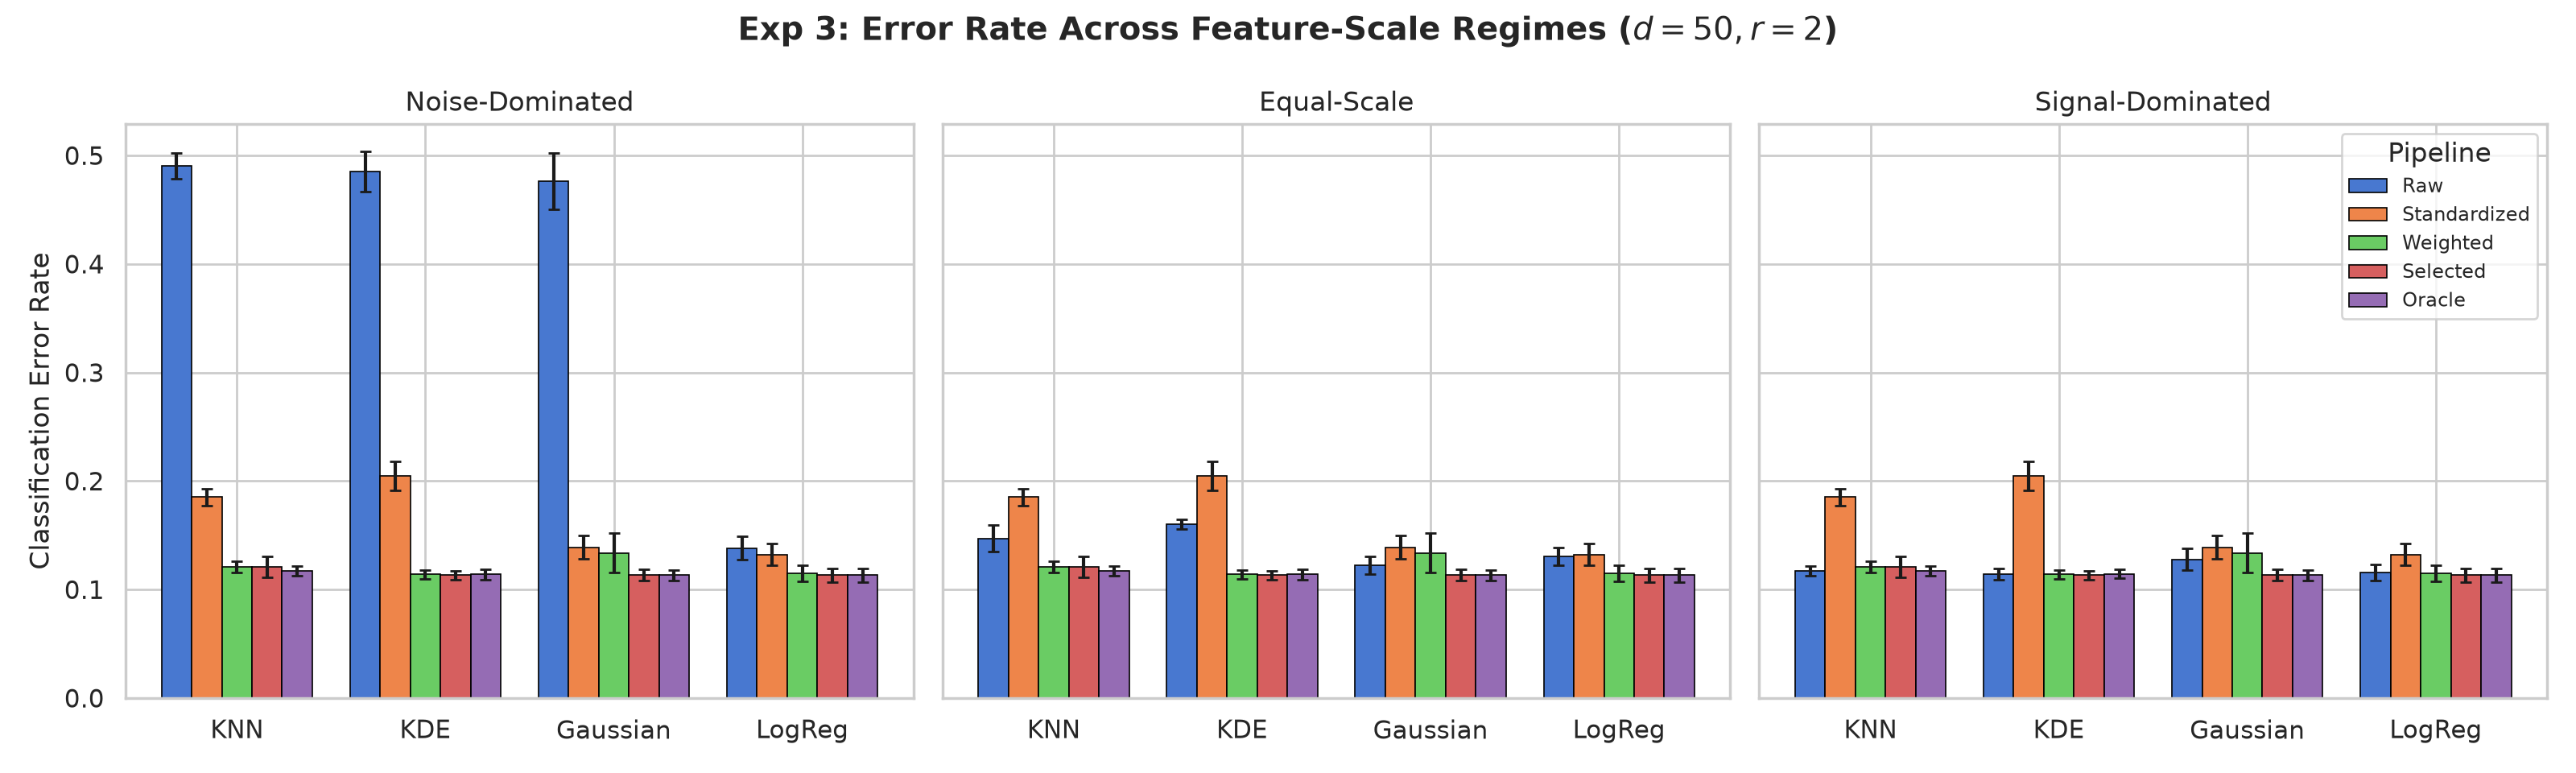
\includegraphics[width=\textwidth]{exp3_error_rate_comparison.png}
    \caption{Experiment 3: Classification error rate across pipelines and scale regimes.}
    \label{fig:exp3_err}
\end{figure}

\begin{figure}[htbp]
    \centering
    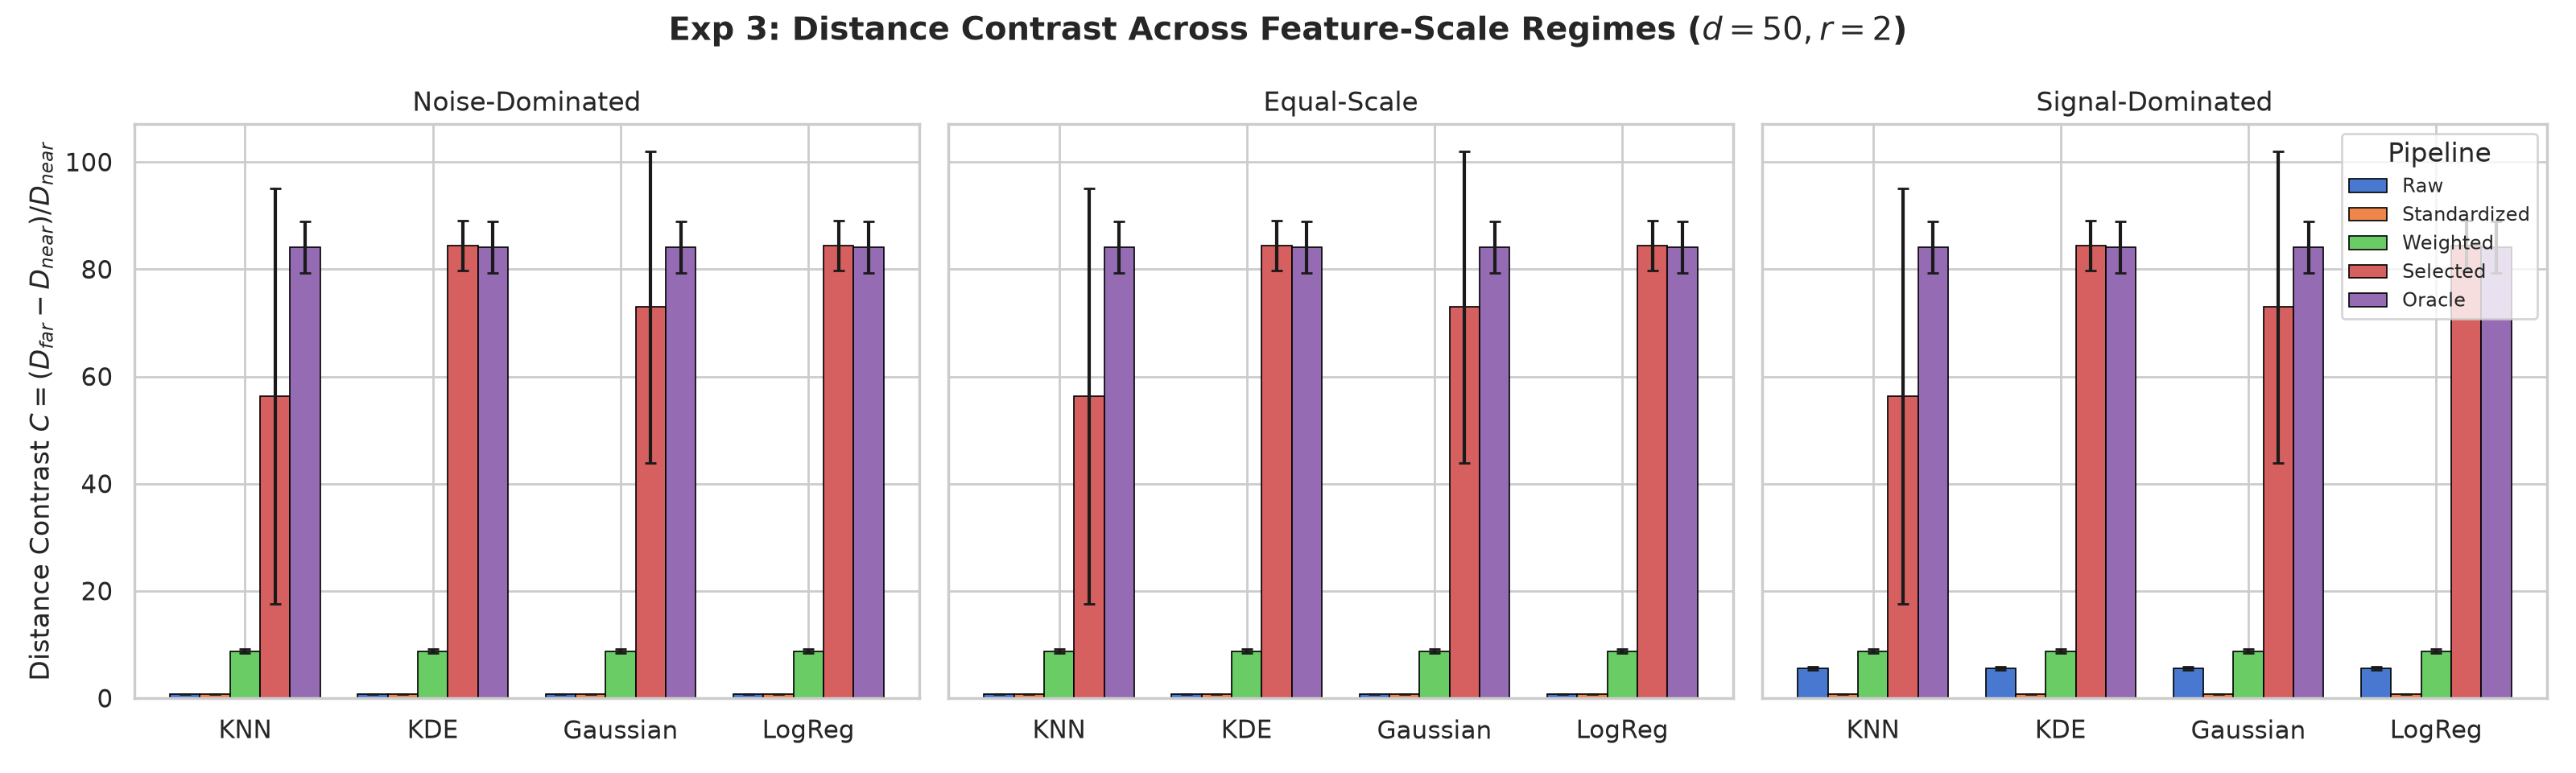
\includegraphics[width=\textwidth]{exp3_contrast_comparison.png}
    \caption{Experiment 3: Distance contrast $C$ across pipelines and scale regimes.}
    \label{fig:exp3_contrast}
\end{figure}

\subsection{When Standardization Helps, Fails, or Hurts}
To understand Table~\ref{tab:exp3} and Figure~\ref{fig:exp3_err}, notice what standardization does to the variances. An irrelevant feature $u_j$ has marginal variance $\sigma_u^2$, so after standardization it has variance $1$. An informative feature $z_j$, however, has marginal variance (across both classes combined)
\[
    \operatorname{Var}(z_j) = \sigma_z^2 + \delta^2 = \sigma_z^2\!\left(1 + \frac{\mu_0^2}{r}\right).
\]
After standardization, the between-class squared-distance gap becomes $\Delta_{\text{std}} = \frac{4\mu_0^2}{1 + \mu_0^2/r} \approx 3.35$ (for $r=2$), while the noise standard deviation is $\sqrt{8(48)} \approx 19.6$, regardless of the original $\sigma_z$ and $\sigma_u$. This explains all three regimes:

\begin{enumerate}
    \item \textbf{Where standardization helps (Noise-Dominated):} On raw data, the 48 noise variables contribute $2(48)(100) = 9600$ to the expected squared distance versus only $4\mu_0^2 = 5.76$ for the class gap. Raw KNN ($49.1\%$), KDE ($48.5\%$), and isotropic-shrunk Gaussian ($47.6\%$) collapse to coin-flipping. (Logistic regression is nearly scale-invariant and stays at $13.8\%$.) Standardization removes the $100\times$ variance imbalance and cuts KNN/KDE error by more than half (to $18.5\%$ and $20.5\%$) and restores Gaussian to $13.9\%$.
    \item \textbf{Where standardization cannot remove irrelevant coordinates (Noise-Dominated \& Equal-Scale):} Even after standardization, all 48 noise dimensions still have variance 1, so distance contrast stays tiny ($C = 0.71$) and KNN/KDE remain far above Oracle ($11.7\% / 11.4\%$). In Equal-Scale, standardizing actually nudges KNN error slightly \textit{up} ($14.7\% \to 18.5\%$) because dividing $z_j$ by $\sqrt{\sigma_z^2 + \delta^2} \approx 1.31$ shrinks the informative features slightly relative to the noise.
    \item \textbf{Where standardization actively hurts (Signal-Dominated):} When the informative features already have a bigger scale ($\sigma_z = 10, \sigma_u = 1$), raw distances naturally focus on $z$ ($C = 5.53$), and Raw KNN ($11.7\%$) and KDE ($11.4\%$) match the Oracle. Standardizing blows the 48 small noise variables up to variance 1, destroying distance contrast ($5.53 \to 0.71$) and pushing KNN error up to $18.5\%$ and KDE error up to $20.5\%$.
\end{enumerate}

Across \textit{all three} regimes, \textbf{Weighted} and \textbf{Selected} pipelines use training labels to down-weight or drop the noise coordinates. As Figure~\ref{fig:exp3_contrast} shows, this restores distance contrast ($C = 8.74$ for Weighted and $56$--$84$ for Selected) and brings all classifiers to $11.3\%$--$12.1\%$ error, matching the Oracle baseline.

% =====================================================================
\section{Experiment 4: Paired Isolation of Informative Dimension ($r$) vs.\ Ambient Dimension ($d$)}

Finally, we separate the effect of the \textit{informative} dimension $r$ from the \textit{ambient} dimension $d$. Keeping $n_{\text{train}} = 500$, $\sigma_z = \sigma_u = 1.0$, and the Bayes error fixed at $11.51\%$ ($\delta = 1.2 / \sqrt{r}$), we vary $r \in \{1, 2, 4, 8, 16, 32\}$ in two paired settings:
\begin{itemize}
    \item \textbf{Fixed Ambient ($d = 50$):} Total dimension stays 50, so increasing $r$ spreads the same total signal over more coordinates while reducing the number of pure noise coordinates ($50 - r$).
    \item \textbf{No Noise ($d = r$):} Zero irrelevant variables; every coordinate is informative, but the same total signal is spread thinly across more dimensions as $r$ grows.
\end{itemize}

\begin{table}[htbp]
\centering
\small
\caption{Experiment 4 mean test error rates and distance contrast $C$ across informative dimensions $r$ (constant Bayes error 11.51\%, $n_{\text{train}}=500$).}
\label{tab:exp4}
\begin{tabular}{lrccccc}
\toprule
Mode & $r$ & KNN & KDE & Gaussian & LogReg & Contrast $C$ \\
\midrule
Fixed Ambient ($d=50$) & 1  & 0.1598 & 0.1688 & 0.1230 & 0.1324 & 0.726 \\
                       & 2  & 0.1472 & 0.1602 & 0.1222 & 0.1306 & 0.725 \\
                       & 8  & 0.1558 & 0.1682 & 0.1278 & 0.1396 & 0.726 \\
                       & 32 & 0.1534 & 0.1562 & 0.1148 & 0.1294 & 0.714 \\
\midrule
No Noise ($d=r$)       & 1  & 0.1194 & 0.1184 & 0.1182 & 0.1184 & 10017.0 \\
                       & 2  & 0.1174 & 0.1140 & 0.1132 & 0.1132 & 84.15 \\
                       & 8  & 0.1292 & 0.1328 & 0.1236 & 0.1244 & 3.75 \\
                       & 16 & 0.1268 & 0.1626 & 0.1146 & 0.1160 & 1.78 \\
                       & 32 & 0.1422 & 0.1324 & 0.1156 & 0.1250 & 0.987 \\
\bottomrule
\end{tabular}
\end{table}

\begin{figure}[htbp]
    \centering
    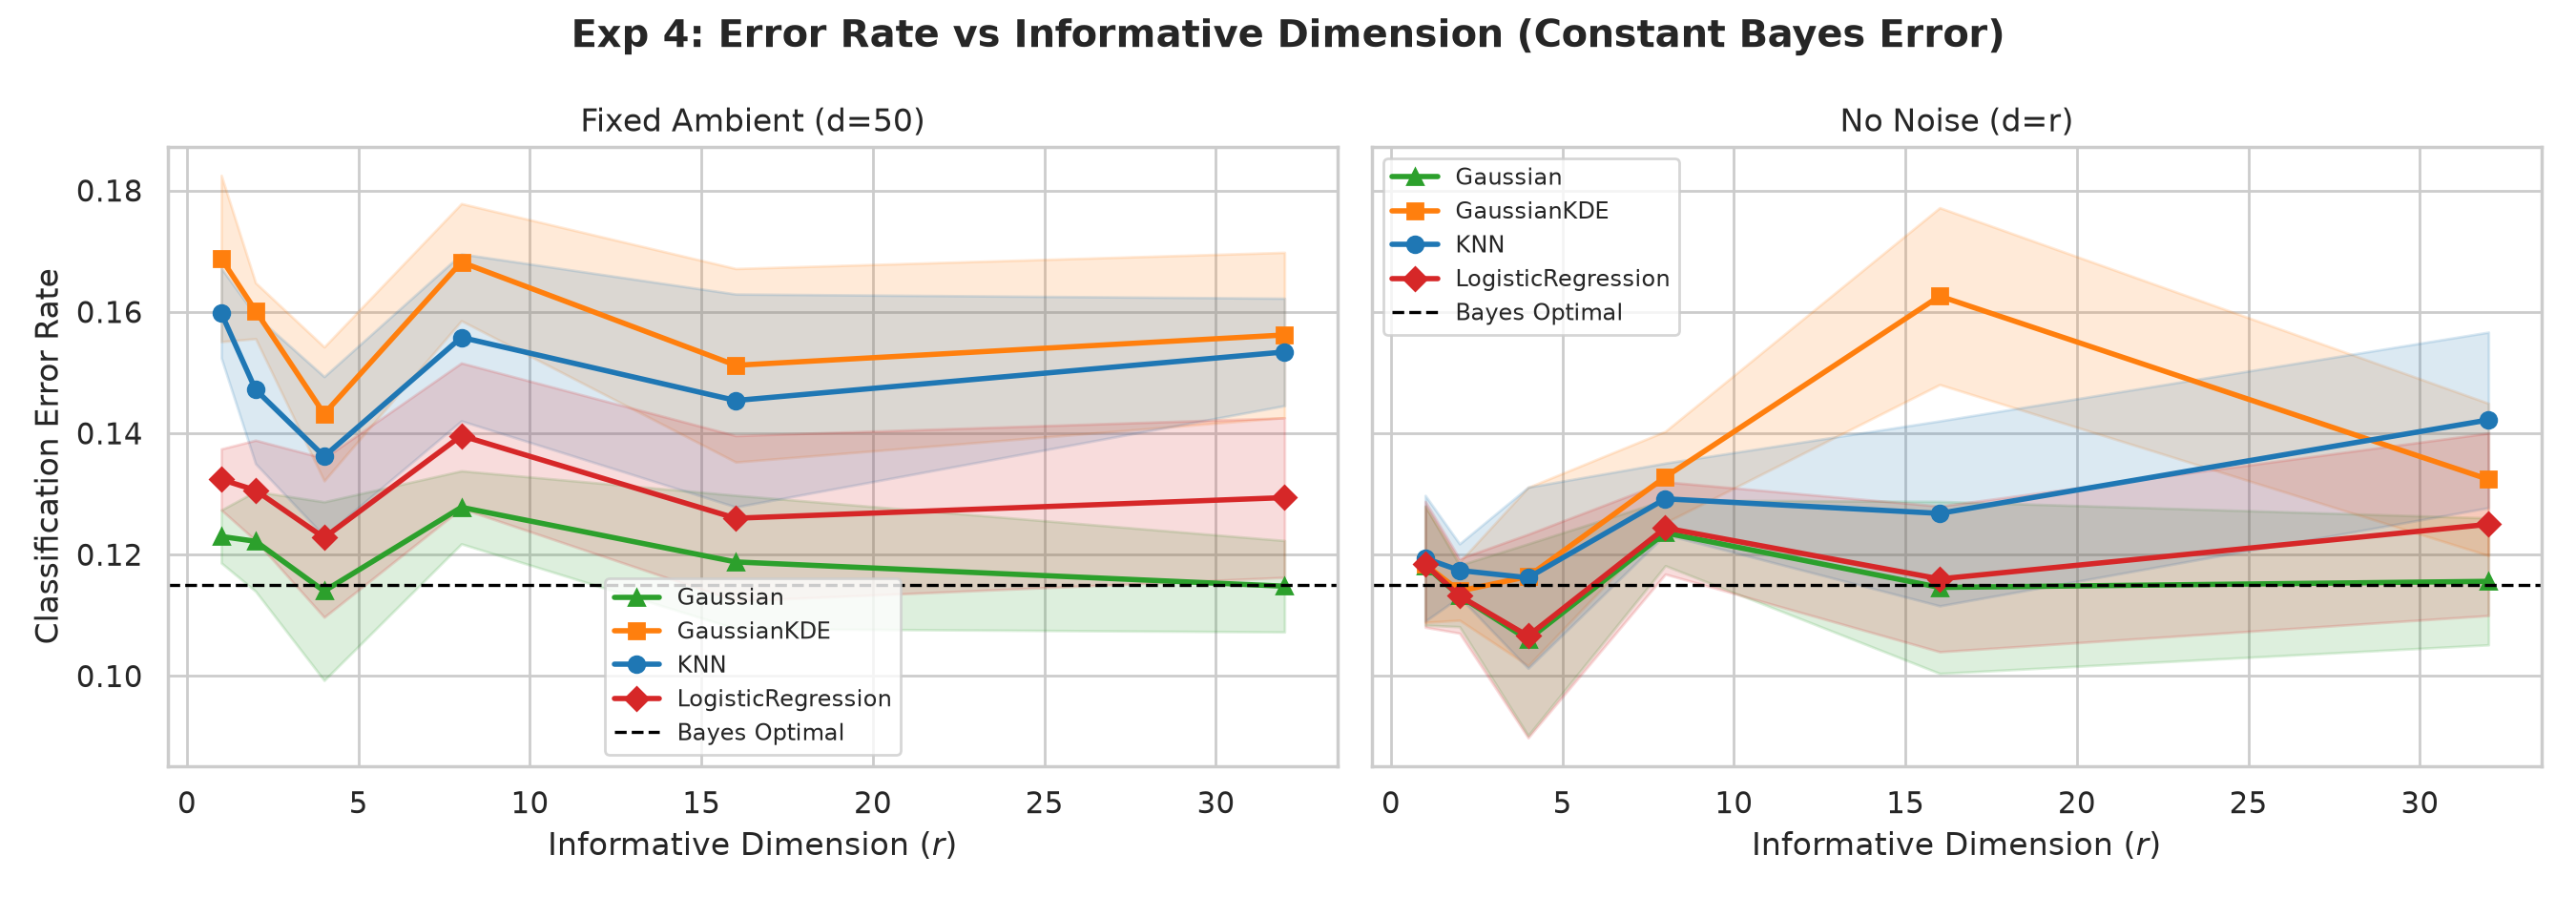
\includegraphics[width=\textwidth]{exp4_error_vs_informative_dim.png}
    \caption{Experiment 4: Error rate vs.\ informative dimension $r$ under Fixed Ambient ($d=50$) and No Noise ($d=r$).}
    \label{fig:exp4_err}
\end{figure}

\begin{figure}[htbp]
    \centering
    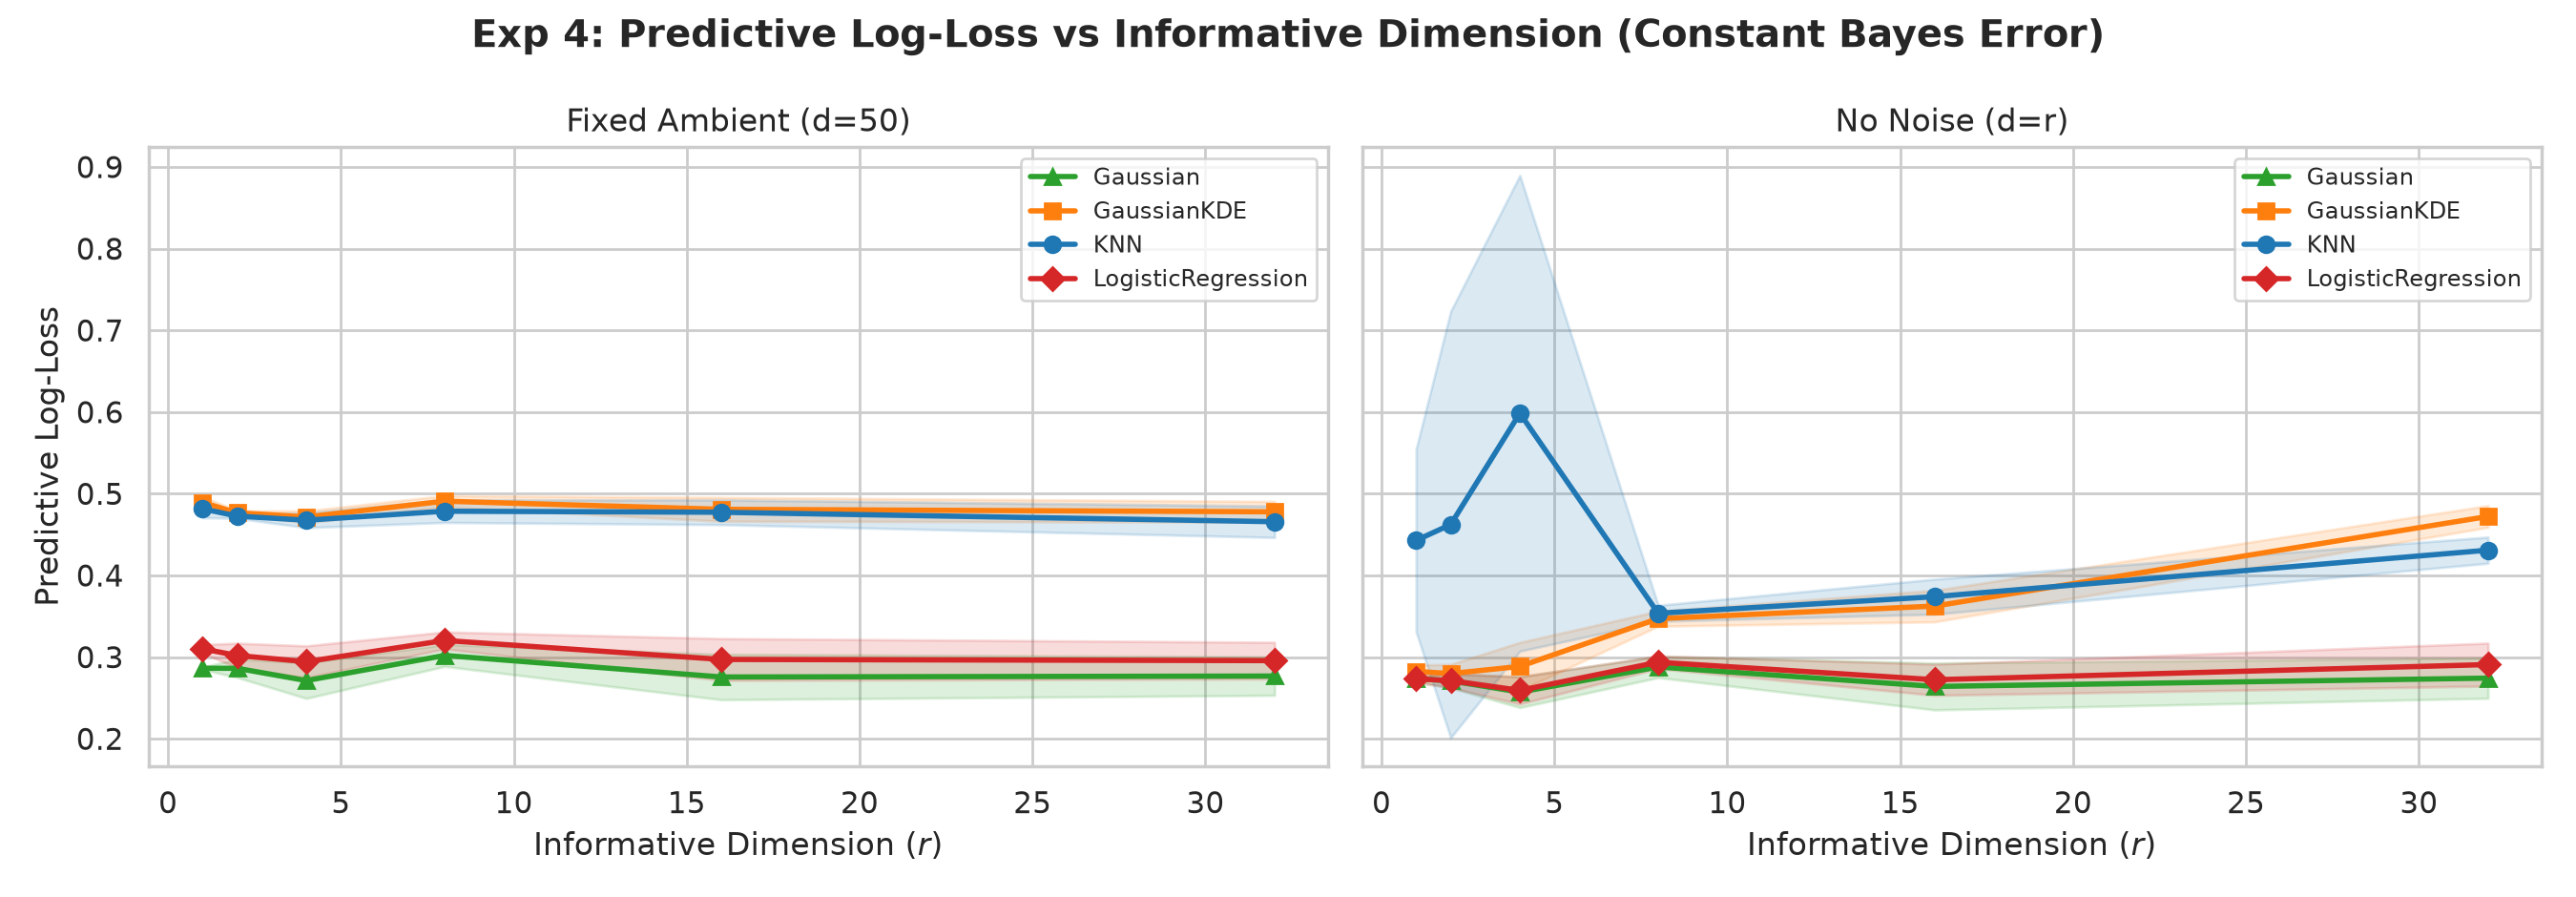
\includegraphics[width=\textwidth]{exp4_log_loss_vs_informative_dim.png}
    \caption{Experiment 4: Predictive log-loss vs.\ informative dimension $r$ under Fixed Ambient ($d=50$) and No Noise ($d=r$).}
    \label{fig:exp4_loss}
\end{figure}

\textbf{Observations:}
\begin{itemize}
    \item \textbf{Fixed Ambient ($d=50$):} Because both total dimension ($d=50$) and total class separation ($2\mu_0 = 2.4$) stay constant, the squared-distance distribution hardly changes ($C \approx 0.72$ everywhere). As seen in Table~\ref{tab:exp4} and the left panels of Figures~\ref{fig:exp4_err} and~\ref{fig:exp4_loss}, error rates and log-losses remain nearly flat across $r = 1 \dots 32$ (KNN $\approx 15\%$, KDE $\approx 16\%$, Gaussian $\approx 12\%$, LogReg $\approx 13\%$).
    \item \textbf{No Noise ($d=r$):} Even with \textit{zero} irrelevant variables, spreading the same signal over more dimensions causes distance contrast to collapse from $10017$ (at $r=1$) down to $0.99$ (at $r=32$). Consequently, KNN error climbs from $11.9\%$ to $14.2\%$, and KDE log-loss climbs steadily from $0.283$ to $0.472$. Meanwhile, Regularized Gaussian and Logistic Regression remain stable near the Bayes floor ($11.6\%$--$12.5\%$).
\end{itemize}

This paired comparison makes an important point: for Euclidean distance-based classifiers, the curse of dimensionality is governed by the \textbf{total dimension $d$} relative to sample size $n$ and total signal strength $\mu_0$---whether the extra coordinates are pure noise (Experiment 1) or dilute the same signal across many informative dimensions (Experiment 4, $d=r$).

% =====================================================================
\section{Conclusion}

Across all four experiments, we see a clear contrast between local distance-based classifiers and regularized parametric classifiers in high dimensions:
\begin{enumerate}
    \item Adding irrelevant features inflates pairwise Euclidean distances and collapses distance contrast $C \to 0$, causing KNN and Gaussian KDE to degrade rapidly while Regularized Gaussian and L2 Logistic Regression remain much more accurate.
    \item Increasing the training sample size by $50\times$ lets parametric classifiers recover the Bayes optimal error ($11.5\%$), whereas KNN and KDE still struggle because high-dimensional space stays sparse.
    \item Standardization is not a cure-all for irrelevant variables. It rescues distance-based models when noise has a much larger scale than the signal, cannot remove unit-variance noise features, and actively hurts when the signal naturally has a larger scale. Supervised feature weighting and training-only feature selection reliably remove noise coordinates and recover Oracle performance in every regime.
    \item When total signal strength is held constant, spreading that signal across many informative dimensions ($d=r$) causes the same distance concentration and local-classifier degradation as adding noise dimensions.
\end{enumerate}

\end{document}
